\documentclass{article}
\usepackage[utf8]{inputenc}
\usepackage{geometry}
\geometry{a4paper, margin=1in}
\usepackage{graphicx}
\usepackage{amsmath}
\usepackage{hyperref}
\usepackage{enumitem}

\hypersetup{
    colorlinks=true,
    linkcolor=blue,
    filecolor=magenta,      
    urlcolor=cyan,
}

\begin{document}

\begin{titlepage}
    \centering
    
    \vspace*{\fill}
    
    % --- Title ---
    {\Huge\bfseries Requirements Specification: \par}
    {\Huge\bfseries Tactile Environment Routing Interface (TERI)\par}
    
    \vspace{2cm}
    
    % --- Author / Group ---
    {\Large Group: Group 5\par}
    \vspace{1cm}
    {\large Francisco Alvarez\par}
    {\large Alejandro Armenta\par}
    {\large Dominic Bertolo\par}
    {\large Carlos Gomez\par}
    {\large Josiah Spann\par}
    {\large Isaac Spann\par}
    
    \vspace{1.5cm}
    
    % --- Date ---
    {\large October 7th, 2025\par}
    
    \vspace*{\fill}
\end{titlepage}

\section{Overview}

\subsection{Purpose}
Tactile Environment Routing Interface (TERI) is designed to address an accessibility gap in complex indoor environments, such as a university campus. The primary purpose is to develop a smart navigation handheld device that provides real-time guidance for users, with a focus on serving students with visual impairments. This device is intended to provide users with a greater sense of independence, safety, and navigational confidence, in doing so reducing the need to rely on sighted guides or memorization of complex routes within buildings.

\subsection{Objective}
The main objective of the project is to deliver a prototype that can successfully guide a user from a starting point to a chosen destination within a pre-mapped indoor area. This project directly aligns with the principles of AI for Social Good (AI4SG) by leveraging technology to increase accessibility and inclusivity of common spaces. TERI intends to reduce barriers and promote a more equitable campus environment for individuals with disabilities by creating a tool that enables equal access to university facilities.

\section{Statement of the Problem}

\subsection{Design Needs}
The primary objective of TERI is the ability to successfully provide navigation of a pre-mapped indoor area. This demands that TERI has reliable indoor positioning that does not implement standard GPS systems as GPS implementations are largely ineffective indoors due to the poor signal communication through the building's construction. This leads TERI to require an indoor localization approach that utilizes points of reference available indoors. Additionally, due to the smaller spaces provided by indoor areas, higher location accuracy is needed than what a standard GPS implementation might provide. The solution requires that TERI utilizes more than one source of reliable information to determine location and will have to implement a hybrid of two methods of localization.

The primary target audience of TERI is users who might have visual impairments. In order for TERI to be intuitive for users, the interface must be completely operable without visual cues. TERI must be functional providing auditory feedback throughout its entire use, from turning on the device to arriving at a user's destination. By not relying on the user to understand the interface through visual cues, the use of the interface must be simple and intuitive physically. TERI will have to implement an interface that is simple and tactile for the user to have constant feedback about how they are using the device.

The intended use case of TERI is to be a portable hand-held design that can be used constantly throughout the day. In order to be handheld and portable, TERI must be battery operated, independent from an external power source for functionality of any kind. Additionally, to be handheld, the form factor for TERI must be comfortable to hold in one hand and be fully navigable with one hand. Additionally, TERI is meant to be easily implemented in an area that has been mapped for navigation. In order to lessen the burden and reliance on external systems being configured, TERI must rely primarily on its own sensors and internalized information to reduce dependence on external sources when possible.

\subsection{Expected Benefits}
The objective of providing visually impaired users with an indoor navigation device promotes their independence. Users with visual impairments often must rely on those around them in order to navigate new and foreign areas. Even with the familiarity of a building or an area, navigating to a new room on a new floor can easily become difficult without the use of visual cues that are often taken for granted. TERI aims to bridge this gap of accessibility of daily navigation for indoor spaces.

While the primary target audience is that of the visually impaired, all users can benefit from TERI. The concept of accessibility is not only for those with a disability or impairment, but the act of making a resource more available to all. TERI acts to bridge a gap of accessibility with a goal of primarily enabling the visually impaired. However, a user who is not visually impaired can utilize TERI to navigate to a new room or area without having to face the anxiety of navigating complex environments or feeling the need to rely on help.

\subsection{Key Considerations}
The cost of materials per unit must be kept low in order to be affordable for individual users, and scalable for universities to implement and distribute to students in mass. Due to the focus of TERI being the functionality and less the visual aesthetic, decisions to cut cost might be made easier if the consequences would be a less visually appealing result. However, a key consideration is also how cost-efficient can the specific hardware that is chosen be made. Ensuring that modules chosen fulfill the expected functionality tests while remaining affordable for construction.

The technical implementation for TERI is a complex hybrid system implementing two user-positioning technologies in order to make a "best of both worlds" solution. One common method of position-tracking being Pedestrian Dead Reckoning (PDR), has a disadvantage that the accumulation of errors over time due to environmental errors. Another common method of position-tracking being Wireless Fingerprinting comes with the disadvantage that it is not highly accurate in determining displacement in small measurements. However, combining these implementations to mitigate the disadvantages of both can result in a PDR system that enables wireless fingerprinting to achieve a significantly higher accuracy (Fernando et al., 2024).

A core part of TERI's design philosophy is that it is primarily reliant on its own systems and internalized information. In the cases that TERI needs to utilize outside resources and systems, it aims to take advantage of existing infrastructure. For the wireless fingerprinting that will be utilized for user-positioning, TERI will utilize the existing WiFi infrastructure, which allows this to be a cost-effective approach to configuring and mapping an area for TERI navigation. Indoor areas will be mapped out to have pre-defined Reference Points (RPs) that will then have the average signal strength over a set amount of time from all visible WiFi Access Points (APs) measured and stored locally on TERI. This will allow a map to be made utilizing the reference points as navigable nodes with the WiFi signal strengths of the APs acting as a form of coordinate system. Additionally, TERI will occasionally check the signal strength coming from the APs and compare it to the stored wireless fingerprints associated with the RPs in order to determine location. Using a k-Nearest Neighbors (k-NN) algorithm, TERI will determine the closest match of the current WiFi signal strength to estimate the user's current location. The use of pre-determined and stored data would mean that certain variables would have to be considered at the time of data collection and data storage. For example, due to the nature of wireless signal interruption, a large presence of people can cause a reduced signal strength. Therefore, data on the average signal strength at a RP must be taken multiple times throughout the day. Then, the time of day is associated with that data as being an expected "high traffic" time period or a "low traffic" time period. The choice of which data set to use is determined by TERI's internal clock that is read at navigation time.

The use of wireless fingerprinting is an auxiliary function to the positioning system. The use of an Inertial Measurement Unit (IMU) for Pedestrian Dead Reckoning will allow for a smooth and continuous tracking of the user's movement between RPs. This allows TERI to calculate and consider additional information to use for navigation including step detection, estimated stride length, and a direction estimation. Benefits from this information, such as step detection and stride length, is that TERI can properly disperse wireless fingerprinting checks across navigation. For example, if two RPs are 20 feet from each other, a wireless fingerprint check is not needed after 2-3 feet travelled. TERI using the IMU can determine when a user has travelled 8-10 feet and wireless fingerprint check to ensure the user is traveling in the correct direction. There is a difficulty when it comes to determining the user's initial direction. In order to remedy this, TERI will implement an increased amount of checks using wireless fingerprinting in order to determine if a user is navigating in the correct direction. If the user is failing to navigate towards the expected direction, they will be corrected based on audio feedback. While this may not be the most intuitive starting experience, it is a design choice to balance complexity of the device with accuracy.

The strength of TERI comes from the hybrid implementation of two powerful user-positioning technologies. The strength of this hybrid approach comes from the implementation utilizing an Extended Kalman Filter (EKF). An EKF is an algorithm used for combining asynchronous and non-linear data in real-time, operating with a predict-update cycle. For TERI's implementation, the prediction will be the use of high-frequency data coming from the IMU in the form of step, stride detection, and heading data to predict where the user is going to be at a given point in time. The update will be the less frequent position estimate that is derived from the wireless fingerprinting check. The EKF will use this wireless fingerprinting check to correct the predicted state, mitigating the accumulated drift from the PDR (Li et al., 2025). However, a key consideration for this implementation is that the inconsistency of wireless fingerprinting or the inconsistency of the wireless fingerprinting correlating to expected results may not mitigate the accumulated error and instead further the error by reinforcing undesired results. Additionally, the use of the IMU and the WiFi module to perform the EKF algorithm, while properly navigating a path that is subject to dynamically change based off of user-driven detours, can result in a difficult power efficiency scenario that can come at the cost of battery-life for TERI.

\section{Operational Description}

\subsection{User's Manual}
\begin{enumerate}
    \item \textbf{Powering On:} To activate the device, slide the "Power" switch on the side of the device upwards. As the device turns on, wait until an audio tone sounds which confirms that the system has successfully powered on and is ready to receive input.
    \item \textbf{Selecting a Destination:} The user will select a destination by entering a unique key code using the different input buttons to select their desired location. For the top two rows of the keypad, each column represents a different section of the keycode. Within these two rows, the above row is to increment the corresponding selection while the below row decrements the same selection.
    \item \textbf{Navigating:} To navigate, the user simply holds on to the device in one hand while following audio cues when provided.
    \begin{itemize}
        \item[a.] A short single beep indicates that the user should continue moving in a straight line.
        \item[b.] A double pulse beep signals that there will be a turn right soon.
        \item[c.] A long beep signals that there will be a turn left soon.
        \item[d.] A rapid sequence of beeps means that the user has arrived at their desired destination.
    \end{itemize}
    \item \textbf{"Where Am I?" Function:} Pressing the button on the bottom left will activate the "Where am I?" feature. When this button is pressed, the device will announce the nearest identifiable RP based on the user's current position, allowing for the user to have a sense of where they are within the environment.
\end{enumerate}

\subsection{User Interface}
TERI is meant to be accessible and easy to use for visually impaired users. Users will use a keypad to input a keycode in the format of A:B:CD, where A is a building or area location represented by 2 letters and B is a floor level represented by a single digit. C and D are paired together to represent the desired room number with C representing the tens-place and D representing the ones-place. This configuration of C and D allows the user to input a room number ranging from 00 to 99 by only navigating two selections ranging from 0 to 9 instead of one selection of 00 to 99. This small change allows the users maximum button presses to reach a room number to decrease from 50 to 10. A, B, C, and D are changeable through the use of the corresponding buttons. Pressing the buttons will cycle through the selections for that variable. After each change, the corresponding location of that keycode is announced through the speaker. Once the user has selected a proper destination, pressing the Go button will ask for confirmation, while pressing it a second time will commence the navigation function.

% Assuming the sketch image from the PDF is saved as 'teri_sketch.png' in the same directory
\begin{figure}[ht!]
    \centering
    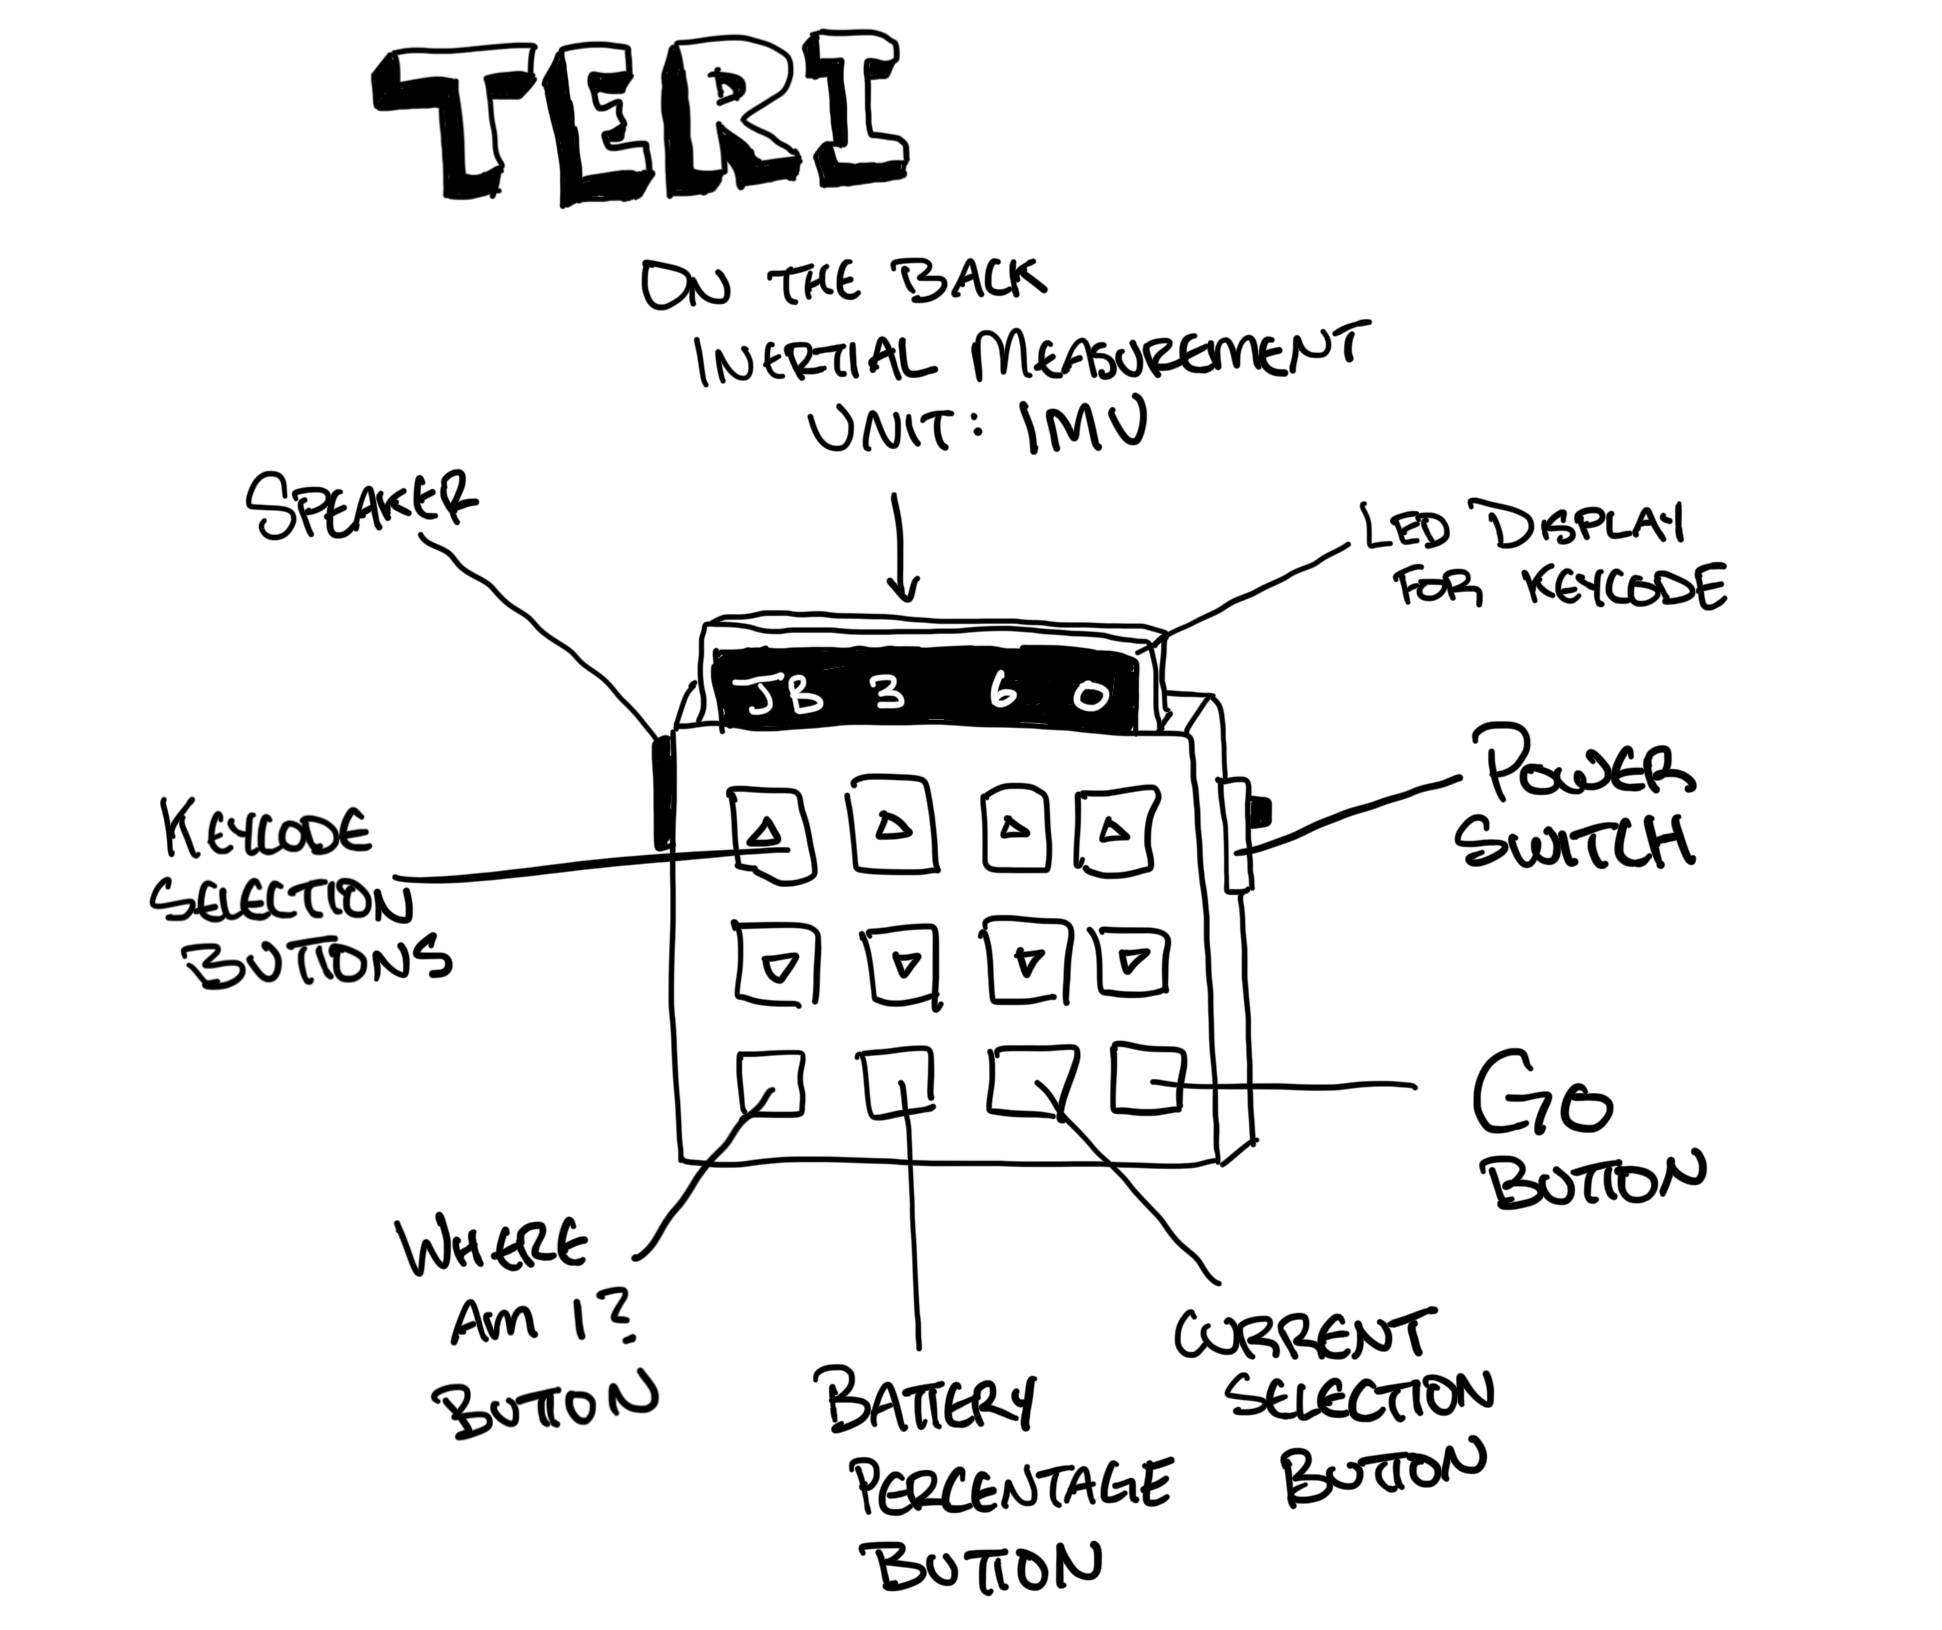
\includegraphics[width=0.8\textwidth]{user_interface_design.png}
    \caption{Sketch of Device (Labeled by Part Functionality)}
    \label{fig:teri_sketch}
\end{figure}

\section{Requirements Specifications}

\subsection{Features and Functions}
With its primary goal of being navigation of an indoor space, TERI's functionality primarily focuses on a simple and intuitive tactile user interface with a complex and reliable user-positioning system. TERI utilizes a hybrid indoor localization system composed of data from an IMU-based PDR fused with data from occasional WiFi fingerprinting checks by an Extended Kalman Filter. This localization technique is then utilized to ensure the user is following a determined path to their desired destination through TERI's pathfinding system. This pathfinding system will utilize the $A^*$ search algorithm to efficiently traverse the pre-defined navigation graph that is composed of the previously mentioned RPs that are also utilized by the user-positioning system.

Along with the complex and reliable user-positioning and navigation system, various user-facing features will be available such as turn-by-turn guidance, a destination menu, and the "Where Am I?" feature. By utilizing the user-positioning system, the user is provided directions to make the correct turns at a given moment. Additionally, they are warned in advance that they will have to make a turn within a set amount of distance. The destination that is selected is defined by the user's input through the physical user interface that is navigated through the use of tactile buttons with auditory feedback. This array of buttons includes a button to trigger the "Where Am I?" feature to allow the user to know where they are based on their proximity to the closest RP detected by the user-positioning system.

\subsection{Input and Output System}
\begin{description}
    \item[User:]
    
    \begin{description}[style=nextline]
        \item[Input:] Tactile button presses for destination selection, "Where am I?", and "GO" requests.
        \item[Output:] Audio cues (speaker) and vibration signals that guide the user during navigation.
    \end{description}
    \item[Control Unit (Raspberry Pi):]
    
    \begin{description}[style=nextline]
        \item[Input:] Data from Initial Measurement Unit (IMU) in the steps taken, estimated stride lengths, estimated direction; Signal strength from pre-mapped WiFi Access Points; User interaction in the form of a keypad and switch.
        \item[Output:] Audio signals to speaker/headphone jack and pathfinding calculations based on the user-positioning system and navigation system, relying on internalized data about average signal strengths of APs at each RP.
    \end{description}
    \item[Sensors:]

    \begin{description}[style=nextline]
        \item[Input:] Sensors will be able to detect physical movement and WIFI signals.
        \item[Output:] Continuous data transmission to the control unit for navigation computations.
    \end{description}
    \item[Power Subsystem:]
    
	\begin{description}[style=nextline]
        \item[Input:] Receives power from a USB-C connection for recharging the internal battery.
        \item[Output:] Supplies voltage to all subsystems while maintaining battery efficiency.
    \end{description}
\end{description}

\section{Design Deliverables}

\subsection{Documented Design}
A finalized documented design of TERI will include its physical construction and its design utilizing 2D and 3D models. 2D models, such as sketches, will provide what the original intended design for functionality was. The 3D models will reflect the more refined design and implementation after the continuous development choices based on choices of hardware or changes of hardware choices throughout the project. Additionally, these 3D models will be more accurate to the scale of TERI and its construction. Included with the hardware depictions in 2D and 3D models, will be the schematic diagrams for the Raspberry Pi modules and how they were used in TERI.

To accompany the hardware implementation and design, there will be corresponding software. Software for TERI will have its source code fully-documented and open-source. There will be a software architecture diagram, along with flowcharts displaying the core logic behind the sensor processing and navigation algorithms. In addition to the documentation about TERI's design in its software and hardware, there will be included a guide on how to properly map an indoor area for TERI to navigate. It will include a step-by-step guide that starts from selecting a floor layout to successfully navigating from point to point within the newly mapped indoor area.

\subsection{Working Prototype}
A fully assembled prototype must be capable of demonstrating all core features as described. Success for demonstrating such core features is determined by the Preliminary System Test Plan. Additionally, while some areas of functionality leave room for acceptable malfunction, some core attributes of TERI's implementation will be artificially stress-tested through the use of software. For example, TERI's navigation system will be tested with various different inputs that may or may not be possible from users and will test TERI on its ability to self-correct its navigation that it guides its users on.

\section{Preliminary System Test Plan}

\subsection{Functionality Test: Pathfinding}
\begin{description}
    \item[Description:] Select a destination from the menu and verify that the device calculates a valid route based on the current user position.
    \item[Success Criteria:] Success is viewed when the device provides the correct instructions within 10 seconds of a destination selection.
\end{description}

\subsection{Functionality Test: User Interface Feedback}
\begin{description}
    \item[Description:] Manually test all the buttons and record feedback responses to confirm that input buttons perform their desired function and that the outputs to those inputs are desired/correct.
    \item[Success Criteria:] Success is viewed when the correct corresponding audio or feedback within a second of each user action.
\end{description}

\subsection{Performance Test: Location Accuracy}
\begin{description}[style=nextline]
    \item[Description:] Place device at 5 pre-defined checkpoints and use the "Where Am I?" function.
    \item[Success Criteria:] The reported location is within a 3-meter radius of the actual location for at least 4 of 5 checkpoints that are tested.
\end{description}

\subsection{Performance Test: Battery Life}
\begin{description}
    \item[Description:] Fully charge the device and run it in a continuous simulation loop and monitor battery performance until shutdown.
    \item[Success Criteria:] Device must be able to operate for at least 2 hours of continuous navigation.
\end{description}

\subsection{Reliability Test: Signal Loss}
\begin{description}
    \item[Description:] Intentionally block the device's ability to see WIFI signals for 15 seconds during navigation to test signal loss.
    \item[Success Criteria:] Device continues to navigate without WIFI signal and resumes WIFI based navigation when available.
\end{description}

\section{Implementation Considerations}

\subsection{Timeline}
\begin{itemize}
    \item \textbf{Weeks 1-2:} Component sourcing, literature review, algorithm design
    \item \textbf{Weeks 3-4:} Physical device configuration (buttons, sensors, battery, etc.), initial software development
    \item \textbf{Weeks 5-6:} Mapping checkpoints and gathering necessary data (distance between checkpoints, average WIFI strength at various times at each checkpoint)
    \item \textbf{Week 7-8:} System testing, debugging, final documentation
\end{itemize}

\subsection{Resources}
\begin{itemize}
    \item \textbf{Hardware:} Access to university electronics labs for testing equipment and possibly 3D printing for custom enclosure, designing it for comfort and feasibility.
    \item \textbf{Software:} Raspberry Pi libraries for sensor integration and audio output. GitHub to be used for version control, collaboration with the team, and source code documentation.
\end{itemize}

\subsection{Potential Challenges \& Mitigation}
One of the core functionalities of TERI is the user-positioning that primarily relies on the IMU-based PDR system. However, these systems are known to be susceptible to accumulating errors over extended use. A solution to this is TERI's implementation of an EKF to fuse the data from the IMU with periodic sanity checks from the WiFi fingerprinting system. However, the issue may persist depending on a low quality IMU unit, where errors may accumulate quicker than can be reliably sanity-checked by a WiFi fingerprinting. A solution to this would be to benchmark the success of navigation with various tweaks to the timings of how often WiFi fingerprinting is requested.

A drawback of TERI is that while it is able to navigate indoor areas with high precision, it is currently labor-intensive to map out and configure an area to be navigable. Additionally, due to the nature of WiFi fingerprinting, different areas would have to be individually configured, not providing a seamless transition for users from pre-defined area to pre-defined area. For the prototype, the solution is to limit the scope to mapping a single, well-defined test area that covers all necessary test cases. A standardized process for future mapping will be included as a step-by-step guide within TERI's design deliverables.

As previously mentioned when discussing the strengths and weaknesses of the IMU-based PDR, it will be difficult to accurately get the estimated direction a user is heading towards if they are stagnant or just started navigation. To remedy this solution, navigation will always guide the user to move forward until receiving enough data to properly determine the current direction of the user and then guide the user the proper direction. While not idealistic for user intuitive design, it remains a design choice made for the sake of simplifying TERI's design and cost.

\section{Attachments and Additional Resources}

\subsection{Materials List and Estimated Costs}
\begin{itemize}
    \item \textbf{Raspberry Pi 4:} \$0 (Included) - \$30
    \item \textbf{Raspberry Pi Power Pack:} \$25
    \item \textbf{4x3 Keypad:} \$10 - \$20
    \item \textbf{Inertial Measurement Unit (IMU):} \$15 - \$25
    \item \textbf{Slide Switch Module:} \$3 - \$5
    \item \textbf{Speaker Module:} \$10 - \$15
    \item \textbf{Total:} \$63 - \$95
\end{itemize}

\subsection{Marketing Studies \& Literature Review}
\begin{description}
    \item[Citation:] Fernando, G. C., Qi, T., Ndimbo, E. V., Abraha, A. T., \& Wang, B. (2025). On Fusing Wireless Fingerprints with Pedestrian Dead Reckoning to Improve Indoor Localization Accuracy. \textit{Sensors, 25}(5), 1294. \href{https://doi.org/10.3390/s25051294}{https://doi.org/10.3390/s25051294}
    \item[Relevance:] This source discusses a core aspect of TERI, being the hybrid approach of two powerful user-positioning technologies and systems. The researchers observed that a hybrid approach dramatically increased the accuracy of positioning systems, with a 30\%+ increase compared to wireless-only systems, and 70\%+ increase compared to PDR only systems. This strengthens the choice to opt for a hybrid approach for TERI, achieving the best of both worlds when it comes to accuracy within the respective ranges of each system.

    \item[Citation:] Li, Z., Tang, Z., Kim, K. S., Li, S., \& Smith, J. S. (2025). EKF-Based Fusion of Wi-Fi/LiDAR/IMU for Indoor Localization and Navigation. \textit{arXiv preprint arXiv: 2509.23118}.
    \item[Relevance:] This source validates the choice of using an Extended Kalman Filter (EKF) as core logic in processing the information from the IMU signals and the WiFi signals. The analysis on EKF in this context is specifically about utilizing WiFi and IMU data for indoor navigation, emphasizing high performance and resiliency with non-linear and relatively unpredictable data like pedestrian movement.

    \item[Citation:] Plikynas, D., Žvironas, A., Budrionis, A., \& Gudauskis, M. (2020). Indoor Navigation Systems for Visually Impaired Persons: Mapping the Features of Existing Technologies to User Needs. \textit{Sensors, 20}(3), 636. \href{https://doi.org/10.3390/s20030636}{https://doi.org/10.3390/s20030636}
    \item[Relevance:] This source provides a broader landscape of assistive technology for indoor navigation. Topics include Bluetooth, cameras, and RFID which can be used to help provide alternative implementation ideas throughout TERI's development. Additionally, it helps add to the perspective of designing TERI to be an accessibility enabling device.

    \item[Citation:] Simões, W. C. S. S., Machado, G. S., Sales, A. M. A., de Lucena, M. M., Jazdi, N., \& de Lucena, V. F., Jr (2020). A Review of Technologies and Techniques for Indoor Navigation Systems for the Visually Impaired. \textit{Sensors (Basel, Switzerland), 20}(14), 3935. \href{https://doi.org/10.3390/s20143935}{https://doi.org/10.3390/s201\-43935}
    \item[Relevance:] This source supports the primary principle that TERI follows that reliance on a single source or system for user-positioning can be unreliable or inaccurate. Results from experimentation documented in the report shows that integration of multiple systems, specifically in the context of sensors and signal processors for localization, is mandatory to build a robust and reliable implementation.
\end{description}

\end{document}